\documentclass{article}
\usepackage[backend=biber, style=apa]{biblatex}
\usepackage{hyperref}
\usepackage{graphicx} % Required for inserting images
\usepackage{amsmath}
\usepackage{amssymb}
\usepackage{enumitem}
\usepackage{geometry}
\usepackage{wrapfig}

\usepackage[table,xcdraw]{xcolor}

\geometry{margin=1in}
\addbibresource{references_find.bib}
\setlength{\intextsep}{0pt} 


\title{Findings}
\author{Anton Mukin}
\date{October 21, 2025}

\setlength{\parindent}{0pt}


\begin{document}

\maketitle

\subsection{Abstract}

\subsection{Introduction}
This project began with a simple idea: a calculator that predicts answers using a neural network rather than performing systematic calculations. The central question that propelled this project was determining the most suitable neural network architecture for this task. This document presents the findings from the "A Predictive Calculator" project.

\subsection{Hypothesis}
Following a \href{https://github.com/AntonStantan/matura/blob/main/zwischenProdukt/LiteraturstudieAnton.pdf}{literature review}, the expected results were as follows: 
It was hypothesized that Feed-forward Neural Networks (FNNs) would be the weakest architecture, Recurrent Neural Networks (RNNs) would perform better, and transformers and pre-trained transformers would perform the best. Technologies such as positional embeddings, a seq2grid pre-processor\footnote{This was skipped because in theory it wouldn't have a big impact if any, mainly only helping with rounding errors.} and a PReLU activation function were expected to help the model generalize simple arithmetic rules.


\newpage
\tableofcontents
\newpage

\subsection{Feed-forward Neural Networks (FNNs)}
The functionality of FNNs has been previously discussed in the literature study and methodology document. As no new information has been found, this topic will not be further discussed here. However, FNNs will be referenced later in this document.

\section{RNN}
Recurrent Neural Networks (RNNs) work similarly to FNNs with one key difference: There is a vector called the hidden-state. This vector contains information about previous inputs. The hidden-state of the previous time-step, in addition to the input of the current time-step, is fed into a model which computes the hidden-state of the present time-step. The output of each time-step is calculated by feeding the respective hidden state to a model.

\subsection{Numerical Visualization of a RNN:}
Let:
\begin{itemize}
    \item $x_t$: Input at time step $t$
    \item $h_t$: Hidden state at time step $t$
    \item $y_t$: Output at time step $t$
    \item $W_{xh}$: Weight matrix connecting input to hidden state
    \item $W_{hh}$: Weight matrix connecting previous hidden state to current hidden state (recurrent weights)
    \item $W_{hy}$: Weight matrix connecting hidden state to output
    \item $b_h$: Bias vector for the hidden layer
    \item $b_y$: Bias vector for the output layer
    \item $\sigma$: Activation function (in our case: PReLU)
    \item $\sigma_{out}$: Activation function for the output (linear for regression)
\end{itemize}

$$h_t = \sigma(W_{xh}x_t + W_{hh}h_{t-1} + b_h)$$
$$y_t = \sigma_{out}(W_{hy}h_t + b_y)$$

\subsection{Relevant Takeaway}
For this project, this means the RNN processes an expression sequentially, one part at a time, rather than as a whole. Due to the nature of the RNN's formula, tokens that appear later in a sequence have a more significant impact on the model's prediction than earlier tokens. This means the output number will almost always be closer to the last number of the expression than the first. This is a common issue with RNNs, not only prevalent in this project. It is more widely known as the vanishing gradient problem.

\section{Other Types of RNNs}
To address the vanishing gradient problem, several architectures have been developed, for example, the Long Short-Term Memory (LSTM) proposed by \cite{6795963}, the Gated Recurrent Unit (GRU) proposed by \cite{cho2014propertiesneuralmachinetranslation} or later, the concept of attention proposed by \cite{bahdanau2016neuralmachinetranslationjointly}.

\subsection{Long Short-Term Memory (LSTM)}
The LSTM architecture solves the gradient vanishing problem by using a memory cell. The model can use this to store \eqref{eq:cell_update_lstm}, forget \eqref{eq:forget_gate_lstm} and pass information from the memory cell to the hidden state \eqref{eq:hidden_state_lstm}.

Let: 
\begin{itemize}
    \item $\sigma(\cdot)$ denotes the sigmoid activation function,
    \item $\tanh(\cdot)$ is the hyperbolic tangent function,
    \item $\odot$ represents element-wise (Hadamard) multiplication,
    \item $[h_{t-1}, x_t]$ is the concatenation of the previous hidden state $h_{t-1}$ and the current input $x_t$,
    \item $W_f, W_i, W_C, W_o$ are trainable weight matrices,
    \item $b_f, b_i, b_C, b_o$ are trainable bias vectors,
    \item $C_t$ is the current memory cell state,
    \item $\tilde{C}_t$ is the candidate cell state,
\end{itemize}

\begin{align}
    f_t &= \sigma\!\left(W_f \cdot [h_{t-1}, x_t] + b_f\right) \label{eq:forget_gate_lstm} \\
    i_t &= \sigma\!\left(W_i \cdot [h_{t-1}, x_t] + b_i\right) \label{eq:input_gate_lstm} \\
    \tilde{C}_t &= \tanh\!\left(W_C \cdot [h_{t-1}, x_t] + b_C\right) \label{eq:candidate_cell_state_lstm} \\
    o_t &= \sigma\!\left(W_o \cdot [h_{t-1}, x_t] + b_o\right) \label{eq:output_gate_lstm}\\    
    C_t &= f_t \odot C_{t-1} + i_t \odot \tilde{C}_t \label{eq:cell_update_lstm}\\
    h_t &= o_t \odot \tanh(C_t) \label{eq:hidden_state_lstm}
\end{align}
Source for the equations: \cite{geeksforgeeks_lstm}
\\[2em]
In the equations you can see the forget gate activation \eqref{eq:forget_gate_lstm}, the input gate activation \eqref{eq:input_gate_lstm}, the candidate cell state \eqref{eq:candidate_cell_state_lstm} and the output gate activation \eqref{eq:output_gate_lstm}.

The cell state is calculated in \eqref{eq:cell_update_lstm}. There, the forget gate which scales the previous cell state is combined with the input gate.

The hidden state is calculated in \eqref{eq:hidden_state_lstm}, where the output activation is applied to the cell state.

\subsection{Gated Recurrent Unit (GRU)}
The GRU architecture works in a similar way to the LSTM. Instead of utilizing memory cells, GRUs directly use the hidden state.

Let:
\begin{itemize}
    \item $\sigma(\cdot)$ is the sigmoid activation function,
    \item $\tanh(\cdot)$ is the hyperbolic tangent function,
    \item $\odot$ denotes element-wise (Hadamard) multiplication,
    \item $[h_{t-1}, x_t]$ is the concatenation of the previous hidden state and current input,
    \item $W_z, W_r, W_h$ are trainable weight matrices,
    \item $b_z, b_r, b_h$ are trainable bias vectors,
    \item $\tilde{h}_t$ is the candidate hidden step
    \item $h_t$ is the current hiddenstep
\end{itemize}

\begin{align}
    z_t &= \sigma\!\left(W_z [h_{t-1}, x_t] + b_z\right) \label{eq:update_gate_gru} \\
    r_t &= \sigma\!\left(W_r [h_{t-1}, x_t] + b_r\right) \label{eq:reset_gate_gru} \\
    \tilde{h}_t &= \tanh\!\left(W_h [r_t \odot h_{t-1}, x_t] + b_h\right) \label{eq:candidate_hidden_state_gru} \\
    h_t &= (1 - z_t) \odot h_{t-1} + z_t \odot \tilde{h}_t \label{eq:update_hidden_state_gru}
\end{align}
Source for the equations: \cite{geeksforgeeks_gru}
\\[2em]
Above you can see the update gate activation \eqref{eq:update_gate_gru}, as well as the reset gate activation \eqref{eq:reset_gate_gru}.

Further down, the reset gate activation is applied to the previous hidden step to calculate the candidate hidden state \eqref{eq:candidate_hidden_state_gru}. 

Lastly the hidden step can be calculated by applying (1 - the update gate activation) to the previous hidden step and combining it with the update gate activation applied to the hidden state candidate \eqref{eq:update_hidden_state_gru}. Depending on whether the update gate activation is larger or smaller, the previous hidden step or the candidate hiddenstate will weigh in more on the current hidden step.

\subsection{Bidirectional LSTM with Attention}
An architecture of this type consists in part of a bidirectional LSTM, meaning two LSTMs working in parallel, one of which processes data from front to back, the other from back to front; their results are then concatenated and passed on.
\\[2em]
The other part of this architecture is the attention mechanism. Here it is, as described by \cite{bahdanau2016neuralmachinetranslationjointly}.

Let:
\begin{itemize}
    \item $\mathbf{h}_t \in \mathbb{R}^{128}$ are the hiddenstates for each timestep $t$, the output from the bidirectional LSTM,
    \item $\mathbf{W} \in \mathbb{R}^{128 \times 128}$ is a trainable weight matrix,
    \item $\mathbf{b} \in \mathbb{R}^{128}$ is a bias vector,
    \item $\mathbf{u} \in \mathbb{R}^{128}$ is a trainable context vector.
\end{itemize}

For each time step $t$, compute:
\begin{align}
    \mathbf{v}_t &= \tanh\!\left( \mathbf{W} \mathbf{h}_t + \mathbf{b} \right) \label{eq:v_bahdanau} \\
    e_t &= \mathbf{u}^\top \mathbf{v}_t \label{eq:attention_score}
\end{align}

Normalize scores using softmax:
\begin{equation}
    \alpha_t = \frac{\exp(e_t)}{\sum_{j=1}^{T} \exp(e_j)} \label{eq:alpha_score}
\end{equation}
The attention weights $\boldsymbol{\alpha} = [\alpha_1, \dots, \alpha_T]$ indicate the importance of each time step.

Then compute the context vector:
\begin{equation}
    \mathbf{c} = \sum_{t=1}^{T} \alpha_t \mathbf{h}_t \label{eq:attention_context}
\end{equation}

Source for equations: \cite{cristina_2023_bahdanau}
\\[2em]
An attention score is calculated for each timestep in \eqref{eq:v_bahdanau}, \eqref{eq:attention_score}, it is then normalized \eqref{eq:alpha_score}. Finally the attention weights scale their respective hiddenstates from the LSTMs, to compute the context vector \eqref{eq:attention_context}.

\section{Transformers} \label{sec:transformers}
The best performing and most widely used architectures for most tasks to date are transformers; they form the basis for LLMs. The key to their success is multi-head self-attention.
\\[2em]
In this document, we will discuss the transformer architecture as first proposed by \cite{vaswani2023attentionneed}.

\subsection{Multi-Head Self-Attention}
\begin{figure}[htbp]
    \centering
    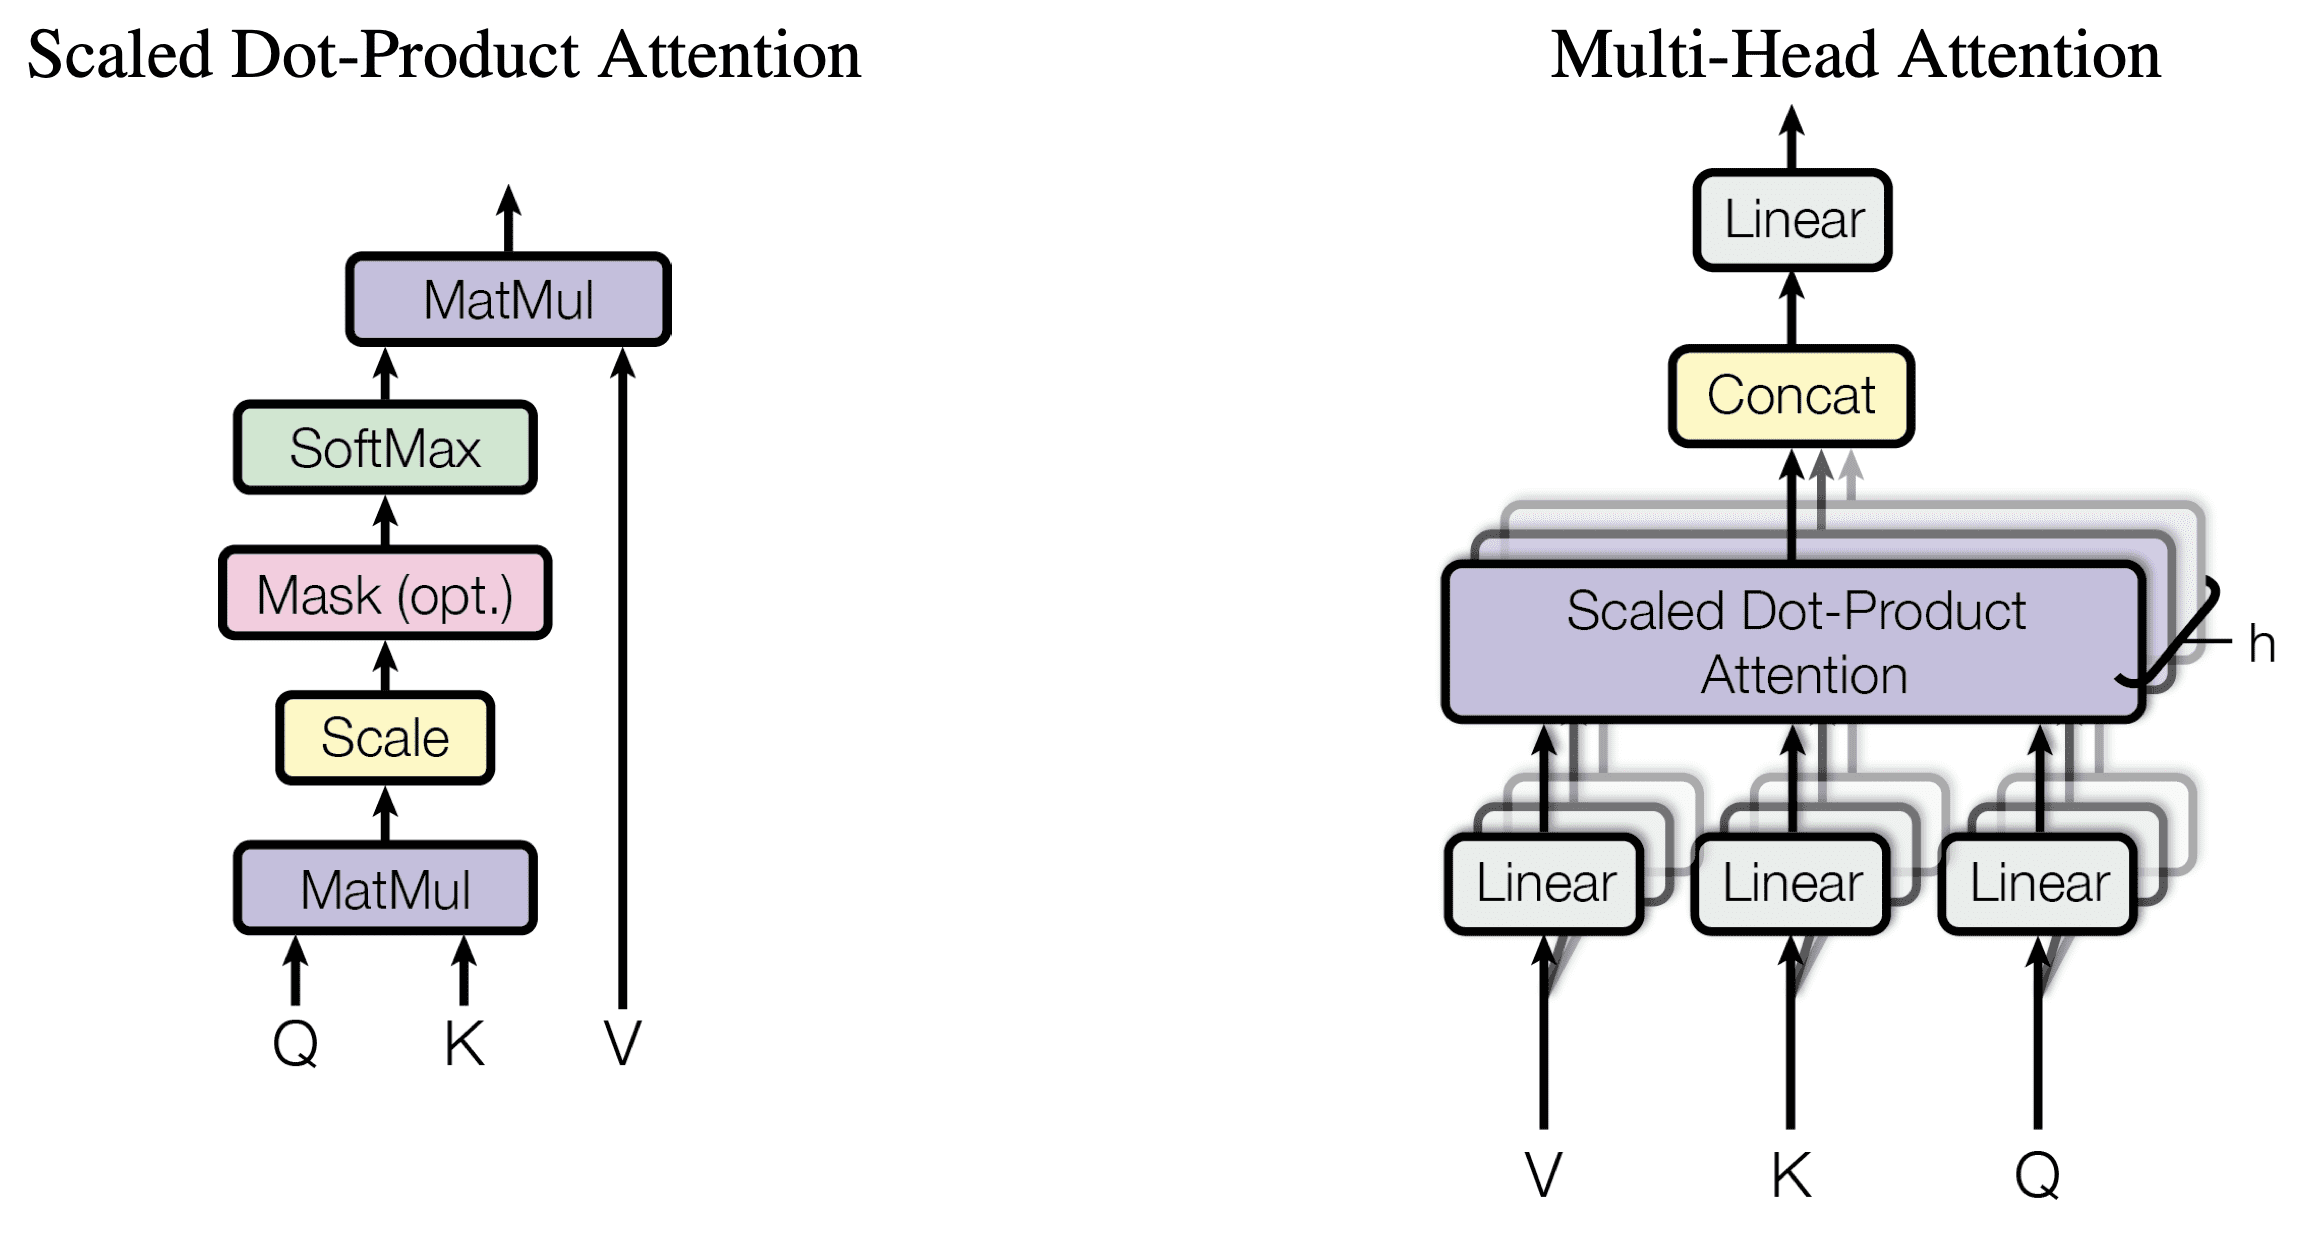
\includegraphics[width=0.5\paperwidth]{images/dotproduct_1.png}
    \caption{Two diagrams from \cite{vaswani2023attentionneed} with the scaled dot-product attention described on the left and multi-head attention on the right.}
    \label{fig:MHAttention}
\end{figure}

Data is first split equally into multiple heads, which process it in parallel. There, the tensors are linearly projected with trainable weights to obtain queries (Q), keys (K), and values (V), which can be seen at the bottom of the image.
$$ Q = X W_Q, \quad K = X W_K, \quad V = X W_V $$
Afterwards, the dot-product between the queries and the keys is calculated and scaled\footnote{According to \cite{vaswani2023attentionneed} this is done to counteract dot-products growing too large and later overwhelming the softmax function.} to determine how similar they are. This leaves us with a number between 0 and 1, representing how much attention to pay. The value $V$ represents the actual information of the token for which we just calculated the attention. This means our final step is to scale the value $V$ by its attention. Pay attention to the equation below. \eqref{eq:sdpAttention}
\begin{equation}
    \text{Attention}(Q, K, V) = \text{softmax}\left( \frac{Q K^\top}{\sqrt{d_k}} \right) V \label{eq:sdpAttention}
\end{equation}

This is done across all heads in parallel. The results are then concatenated\footnote{This means they are reassembled to have the same dimensions as before they were split up.} back together and they undergo a linear projection. As described below:
\begin{gather*}
\text{MultiHead}(Q, K, V) = \text{Concat}(\text{head}_1, ..., \text{head}_h) W^O \\
\text{where: } \text{head}_i = \text{Attention}(Q W_i^Q, K W_i^K, V W_i^V)
\end{gather*}

\newpage
\subsection{The Encoder Layer}
\begin{wrapfigure}{l}{0.3\textwidth}
    \centering
    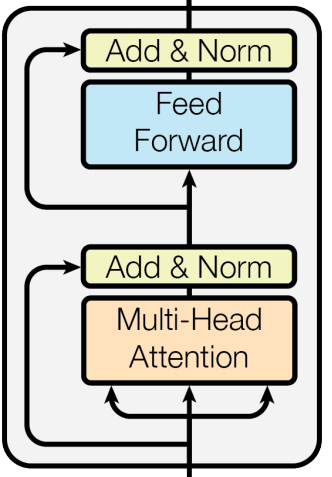
\includegraphics[width=0.2\paperwidth]{images/encodingLayer.png}
    \caption{Encoder Layer as described by \cite{vaswani2023attentionneed}}
    \label{fig:encodingLayer}
\end{wrapfigure}
In figure \ref{fig:encodingLayer} the multi-head attention first undergoes a residual connection as well as a layer normalization \footnote{Given an input vector, layer normalization works by normalizing its features and making it so their mean is 0.}, as described below:
\begin{gather}
    \text{where Sublayer(x) is the function the residual connection is formed around:} \nonumber \\
    \text{Output}(x) = \text{LayerNorm}\bigl(x + \text{Sublayer}(x)\bigr) \label{eq:ResConnect}
\end{gather}
Afterwards, all tokens are fed into a point-wise FNN, where they are processed separately and independently. This part is crucial, to introduce non-linearity into the system, as multi-head attention is linear, and non-linearity is needed for a model to be able to learn.

\subsection{Point-wise Feed-Forward Network}
Equation \eqref{eq:pointwiseFNN} and figure \ref{fig:pointwiseFNN}:
The pointwise FNN works by taking in a number of $d\_model$ tokens, then a layer with a number of $d\_FNN$ neurons with weights and biases $W_1$ and $b_1$ is applied to them individually. The activation function ReLU discards all negative vlaues and the output layer with weights and biases $W_2$ and $b_1$ resets the data back to it's original dimensionality.
After undergoing a residual connection and layer normalization like after multihead attention \eqref{eq:ResConnect}, this makes up a single layer of the Encoder.
A regressive transformer model, like the one used in this project, consists of multiple such encoding layers and last but not least a FNN with a single neuron, which works as the output layer.
\begin{equation}
    \text{pointwiseFNN}(x) = \max\bigl(0, \, x W_1 + b_1 \bigr) W_2 + b_2 \label{eq:pointwiseFNN}
\end{equation}
\begin{figure}[htbp]
    \centering
    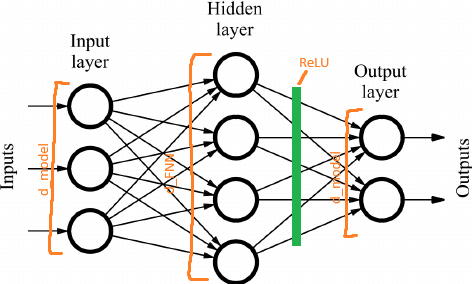
\includegraphics[width=0.4\paperwidth]{images/pointwiseFNN.png}
    \caption{A diagram representing the structure of a pointwise FNN. \href{https://datascience.stackexchange.com/questions/68020/what-is-the-feedforward-network-in-a-transformer-trained-on}{source for figure}}
    \label{fig:pointwiseFNN}
\end{figure}

\subsection{Positional Encoding}
A special characteristic of the transformer is that data is passed through it as a whole. This means the model does not have positional understanding on its own. To counteract this effect, a positional encoding is applied to the input sequences after the tokenizer.

\newpage
\section{Fine-Tuned Pre-Trained LLMs}
The last model type used for this project are fine-tuned Large Language Models (LLMs).
For sources and further reading on this section see (in chronological order; left to right): \cite{geeksforgeeks_2024,Stryker_LLM,srinivasan2024transformer,Bergmann_Fine_Tuning}

\subsection{LLM}
LLMs adopt the transformer architecture\footnote{The transformer architecture discussed in the previous section \ref{sec:transformers}. It not only consists but also a decoder, which is responsible for the model's output} and adapt it to imense sizes, by increasing the architecture's hyperparameters, as well as employing new technological advancements. The number of parameters used by a LLM varies from model to model, but lies in the hundreds of billions per popular high-end LLM.
The large size allows large architectures to excell at complicated tasks like mostly Natural Language Processing (NLP).
To facilitate training and prediction on such large architectures, massive supercomputers are used, consisting of thousands of GPUs. They mainly work by utilizing parallel processing to distribute the load across multiple powerful GPUs. While by far not a supercomputer, a tiny replica was used for this project: The Nvidia Jetson Orin Nano Super Developer Kit.

\subsection{Fine-Tuning Process}
Most of the time LLMs are trained on huge dumps of unlabeled data, which we call unsupervised, or on unlabelled data from which ground truth can be inferred, which we call self-supervised data. 
The fine-tuning process on the other hand is mostly done on smaller datasets with supervised data, meaning it is labeled.
\\[2em]
In the fine-tuning process, a pre-trained model, with its weights and biases already optimized, is trained again on additional data. This means that the model's weights will be slightly adjusted from their pre-trained state. The optimizer will find a new minimum in which the model will have learned additional information from the fine-tuning training data. When evaluated on test data, the newly fine-tuned model is expected to perform better than its pre-trained counterpart.

\subsection{In Addition}
Please note that these are not regression models but sequence-to-sequence models, which means that inside the model, tokens are processed, not numbers, as in the other models discussed. For the task in this project, specifically, fine-tuned models will output an integer rather than a float, because tokens for floats have not been created. This is the reason why the only metric that makes sense for these models is accuracy, which essentially evaluates how many times the model predicted correctly.

\newpage

\section{Findings}
Lastly, the most noteworthy architectures were evaluated and scored on a benchmark. The results were documented in this table: 
\\[0.5em]
\begin{table}[htbp]
\centering
\footnotesize
\begin{tabular}{|lr|r|r|r|r|r|r|}
\hline
\multicolumn{2}{|l|}{Regression models:}                              & \multicolumn{1}{l|}{FNN2} & \multicolumn{1}{l|}{FNN3}        & \multicolumn{1}{l|}{RNN2} & \multicolumn{1}{l|}{Bidirectional   LSTM} & \multicolumn{1}{l|}{transformer4} & \multicolumn{1}{l|}{transformer5} \\ \hline
\multicolumn{2}{|l|}{Total   Parameters:}                             & 6’211                     & 8’893                            & 222’464                   & 19’535                                    & 114’628                           & 1’494’724                         \\
\multicolumn{2}{|l|}{Architecture   Parameters:}                      & 6’211                     & 8’893                            & 222,464                   & 6’511                                     & 38’209                            & 498’241                           \\
\multicolumn{2}{|l|}{Optimizer   Parameters:}                         & -                         & -                                & -                         & 13’024                                    & 76’419                            & 996’483                           \\
\rowcolor[HTML]{F7C7AC} 
MAE in Range:                              &                          & 0.0389406                 & 0.034600                         & 0.2730647                 & 0.5908327                                 & 0.0448075                         & 0.0381983                         \\
\rowcolor[HTML]{F7C7AC} 
MRE in Range:                              &                          & 0.0155504                 & 0.013438                         & 0.1135200                 & 0.2712299                                 & 0.0188047                         & 0.0151836                         \\
\rowcolor[HTML]{94DCF8} 
MAE out Range:                             &                          & 2.2301364                 & \cellcolor[HTML]{83CCEB}2.504607 & 3.5727410                 & 3.2350100                                 & 4.5702314                         & 4.9287004                         \\
\rowcolor[HTML]{94DCF8} 
MRE out Range:                             &                          & 0.2509270                 & \cellcolor[HTML]{83CCEB}0.290885 & 0.3472042                 & 0.3404062                                 & 0.5201459                         & 0.5431157                         \\
\rowcolor[HTML]{FFDC6D} 
\multicolumn{2}{|l|}{\cellcolor[HTML]{FFDC6D}MAE   long Expressions:} & 6.2929916                 & 6.116872                         & 6.0766930                 & 2.7806435                                 & 6.1630590                         & 6.0680327                         \\ \hline
\rowcolor[HTML]{D86DCD} 
\multicolumn{2}{|l|}{\cellcolor[HTML]{D86DCD}Benchmark   score:}      & 6.6345832                 & 6.672521                         & 0.4793787                 & 1.7374969                                 & 2.8882827                         & 5.2896368                         \\ \hline
\end{tabular}
\end{table}

And the fine-tuned Language Models, evaluated on their accuracy:
\\[0.5em]
\begin{table}[htbp]
\centering
\footnotesize
\begin{tabular}{|ll|l|l|l|}
\hline
\multicolumn{2}{|l|}{fine-tuned Language Models:}                          & Gemini 2.5 Pro & Gemma 3 1B & Gemma 3 270M \\ \hline
Parameter size:                               &                            & 1.4E+11        & 1.00E+09   & 2.70E+08     \\
\rowcolor[HTML]{F7C7AC} 
\multicolumn{2}{|l|}{\cellcolor[HTML]{F7C7AC}Accuracy   in Range:}         & 95.17          & 93.41      & 54.22        \\
\rowcolor[HTML]{94DCF8} 
\multicolumn{2}{|l|}{\cellcolor[HTML]{94DCF8}Accuracy   out Range:}        & 99.51          & 63.33      & 9.67         \\
\rowcolor[HTML]{FFDC6D} 
\multicolumn{2}{|l|}{\cellcolor[HTML]{FFDC6D}Accuracy   long expressions:} & 90             & 39.57      & 28           \\ \hline
\end{tabular}
\end{table}

Firstly, it is notable that the main hypothesis of the thesis—that more complex models would perform better—is not supported by the results. There are clear outliers, such as the outstanding performance of the FNN2 or the poor performance of the RNN2 model. Also, notice the minimal improvement between FNN2 and FNN3, which includes a positional embedding layer. The FNN models show the best performance on the benchmark, meaning they are crowned the winners.

\section{Discussion}
\subsection{Regression Models}
All of the 3 or 4 architectures discussed here are very different, and all of them have different strengths and weaknesses, as you can tell by their performances on different sets of test data. Recurrent Neural Networks excel at long expressions, due to the way data is passed through these models sequentially in hidden steps. They are designed for handling longer inputs. Similarly, Bidirectional LSTMs with attention are even more effective when adjusting to a longer input. They can confidently predict longer expressions the best out of all the models studied in this project. This is because vanishing gradients are punished heavily when solving arithmetic expressions by nature, and this model combats this well, as opposed to the simplistic RNN architecture. Additionally, the attention mechanism not only helps with vanishing gradients in longer expressions but also emphasizes outstandingly large numbers and their corresponding signs. When it comes to transformers, they perform best on data just like the one they are trained on, but not exactly the same—the classical definition of validation data. There are too many different types of different parameters, which all have been trained to process training data; this means even the smallest differences in input will lead to the model processing them wrong. Thanks to positional encoding, transformers can handle longer inputs better than FNNs. The FNN architecture performed with the best benchmark. While its ability to generalize laws is bad, the FNN2 model was good at expressions of the same length with numbers not encountered in the training data. Even after adding positional embedding in FNN3, the model struggles at grasping expressions of different sizes.

\subsection{Pre-trained Fine-tuned Transformers}
The models in the table below are all very large, with Gemini 2.5 being particularly massive. Because we know that these models have the same transformer architecture and the sweet spot for hyperparameters is much smaller than their parameter size, we expect a weaker performance.\footnote{Since these are seq2seq models, their hyper-parameters sweet-spot wouldn't be the same as the regression transformers. And their Decoder multiplies the number of parameters roughly by 2x. This is still not comparable to the jump in complexity between the largest optimized transformer regression model and the smallest pre-trained model, which is a factor of 180x.}. Additionally, they predict on tokens rather than numerical values, which is not optimal for the task in this project. The performance of these models also depends heavily on the pre-training they previously underwent because it also involves arithmetics. This explains why the bigger pre-trained models perform better. The Gemini 2.5 Pro model performed the best out of all models evaluated in this project on generalization tests, but this is due to previous training, including expressions similar to those in the training data.

\subsection{Conclusion}
Adding positional embedding barely makes a difference for FNNs.
RNNs are weak models, outclassed by bidirectional LSTMs with attention, and should not be used.
Transformers excel at accurately learning the training data but struggle with generalization more than other models.
FNNs are, overall, the best at generalizing and perform best on the defined benchmark. They are the best architecture for solving simple arithmetic expressions with a reasonable supply of computational resources.
If maximum performance with unlimited computational resources is the goal, a fine-tuned, cutting-edge pre-trained model such as Gemini 2.5 Pro will yield the best results.

\subsection{Possible Future Work}
The topic chosen for this project is very grand and current. A logical and important continuation of this project is using the benchmark as the loss function; this might lead to the training of better-performing models. Another possible direction is improving models by evaluating different activation functions, optimizers, or training data and using the best one, or even designing one's own. Training data and its tokenizer and padding is an area with lots of potential for improvement, i.e., by using an additional embedding. Also, consider this a proposal to evaluate a model architecture: an FNN with attention seems to be promising. Judging by the results in this study, this model is expected to improve the FNN's performance with longer expressions than in training, as well as strengthen its ability to accurately and confidently predict test data inside of the number range, previously referred to as the classical validation data.

\newpage
\printbibliography[heading=bibintoc]
\end{document}